\subsection{Motivation}

\begin{frame}{Introduction}
  \begin{itemize}
      \item Consider a statistical model where we have observations $\by = (y_1, \dots, y_n)$ and also some latent variables $\bz = (z_1, \dots, z_m)$.
    \pause  
    \item Want to evaluate the intractable integral
    \[
      \cI := \int p(\by|\bz)p(\bz) \d\bz
    \]
    \begin{itemize}
      \item Bayesian posterior analysis
      \item Random effects models 
      \item Mixture models
%      \item etc.
    \end{itemize}
%    \item Possible ways: quadrature methods, Laplace approximation, MCMC
    \item Variational inference approximates the ``posterior'' by a tractably close distribution in the KL sense.
    \item Advantages:
    \begin{itemize}
      \item Computationally tractable
      \item Convergence easily assessed
      \item Works well in practice\footnote{With some caveats which will be discussed.} 
    \end{itemize}
  \end{itemize}
\end{frame}

%\subsection{The variational principle}
%
%\begin{frame}{The variational principle}
%  \vspace{-10pt}
%  \begin{itemize}[<+->]
%    \item Name derived from calculus of variations which deals with maximising or minimising functionals.
%    \begin{table}
%      \begin{tabular}{l  l  l }
%      Functions   &$p:\theta \mapsto \bbR$  &(standard calculus) \\ 
%      Functionals &$\cH:p \mapsto \bbR$     &(variational calculus) \\ 
%      \end{tabular}
%    \end{table}
%  \item Using standard calculus, we can solve
%  \[
%    \argmax_\theta p(\theta) =: \hat\theta
%  \]
%  e.g. $p$ is a likelihood function, and $\hat\theta$ is the ML estimate.
%  \item Using variational calculus, we can solve
%  \[
%    \argmax_p \cH(p) =: \tilde p
%  \]
%  e.g. $\cH$ is the entropy $\cH = - \int p(x)\log p(x) \d x$, and $\tilde p$ is the entropy maximising distribution.
%  \end{itemize}
%  \vspace{5pt}
%\end{frame}

\begin{frame}{In the literature}
  \vspace{-15pt}
  \begin{figure}[h]
    \hspace{-15pt}{\color{white} a}
    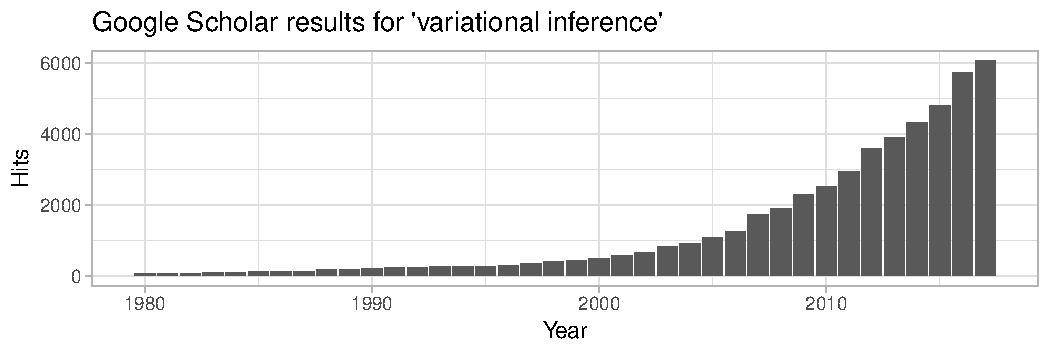
\includegraphics[scale=0.69]{google_scholar}
  \end{figure}
  \vspace{-15pt}
  \begin{itemize}
    \item Well known in the machine learning community.
    \item In social statistics:
    \begin{itemize}\footnotesize
      \item \fullcite{erosheva2007describing}
      \item \fullcite{grimmer2010introduction}
      \item \fullcite{wang2017}
%      \item \fullcite{westling2017}
    \end{itemize}
  \end{itemize}
\end{frame}

\begin{frame}{Recommended texts}
  \begin{itemize}
    \item \fullcite{beal2003}
    \item \fullcite{Bishop2006}
    \item \fullcite{Murphy1991}
    \item \fullcite{blei2017variational}
  \end{itemize}
\end{frame}

\begin{frame}{Idea}
  \blfootnote{\fullcite{bleiyoutube}}
  \vspace{-45pt}
  \begin{figure}[t]
    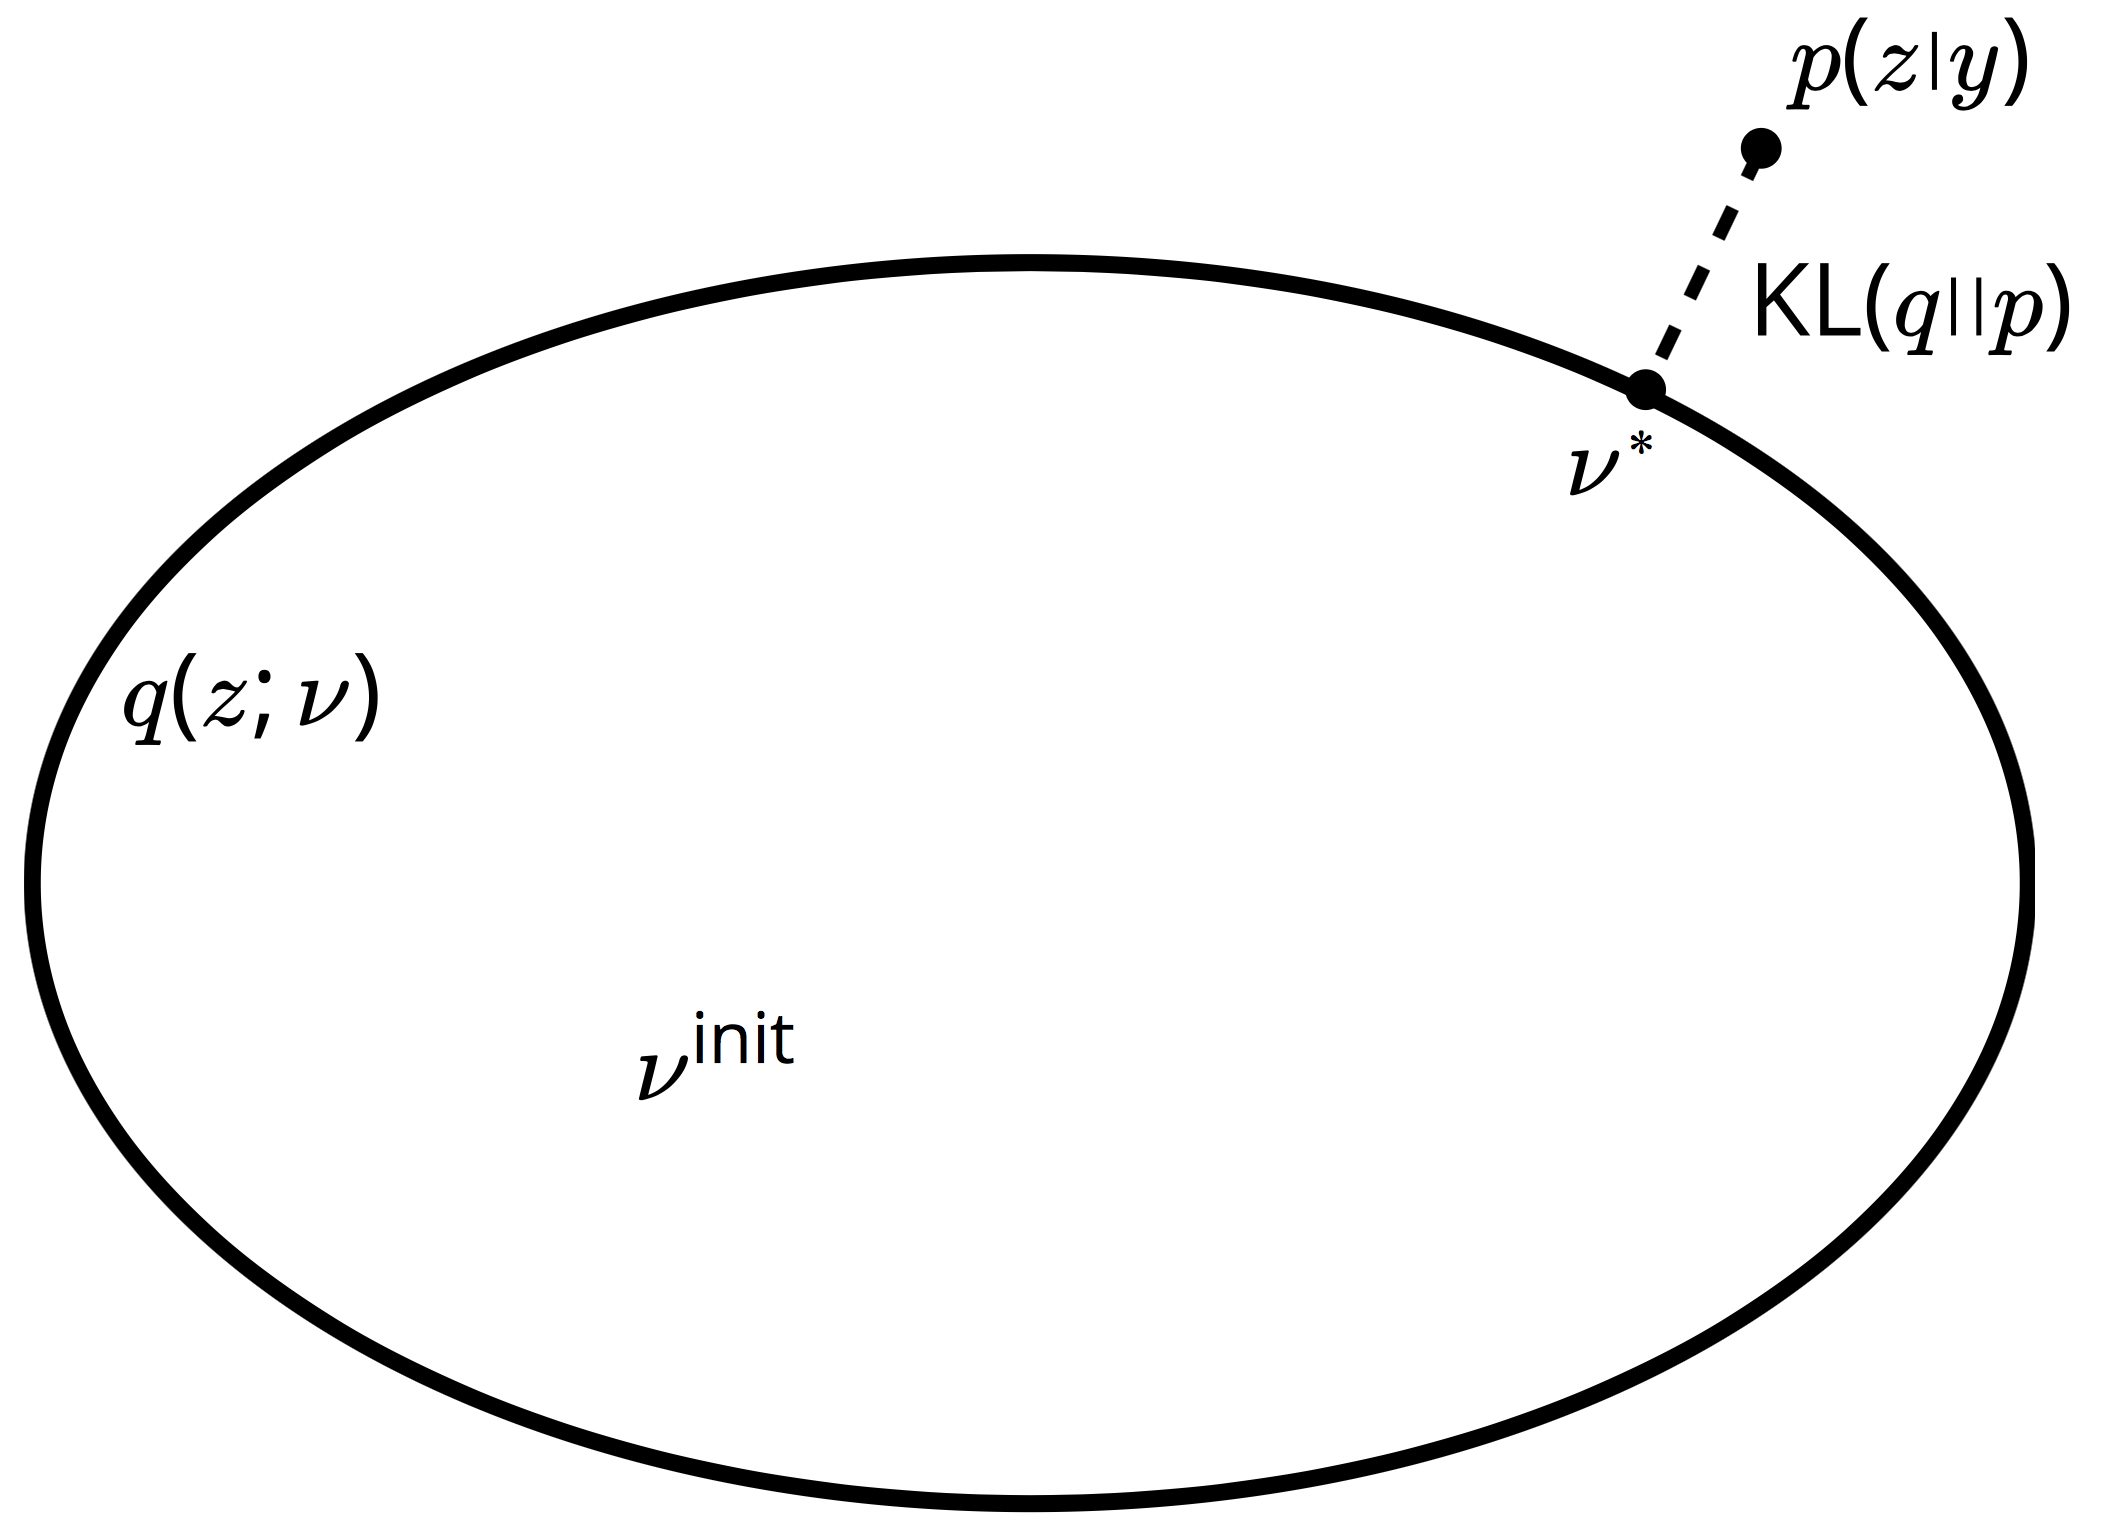
\includegraphics[scale=0.2]{figure/variational_pictorial}
  \end{figure}
  \vspace{-9pt}
  \begin{itemize}
    \item Minimise Kullbeck-Leibler divergence using calculus of variations
    \[
      \KL(q \Vert p) = -\int \log \frac{p(\bz|\by)}{q(\bz)} q(\bz) \d\bz
    \]
%    \item Minimisation of $\KL(q\Vert p)$ is a problem of calculus of variations.
    \item \textbf{ISSUE}: $\KL(q\Vert p)$ is intractable.
  \end{itemize}
\end{frame}

\begin{frame}{The Evidence Lower Bound (ELBO)}  
  \vspace{-3pt}
  \begin{itemize}\setlength\itemsep{0.5em}
    \item Let $q(\bz)$ be some density function to approximate $p(\bz|\by)$. \pause Then the log-marginal density can be decomposed as follows:
    \begin{align*}
      \log p(\by) &= \log p(\by,\bz) - \log p(\bz|\by) \\
      \onslide<3->{
      &= \int \left\{ \log \frac{p(\by,\bz)}{q(\bz)} - \log \frac{p(\bz|\by)}{q(\bz)} \right\} q(\bz) \d \bz \\    
      &=  \cL(q) +  \KL(q \Vert p) \\
      &\geq \cL(q) 
      }   
    \end{align*}
    \item<4-> $\cL$ is referred to as the ``lower-bound'', and it serves as a surrogate function to the marginal.
    \item<4-> Maximising $\cL(q)$ is equivalent to minimising $\KL(q \Vert p)$.
    \item<4-> \textbf{ISSUE}: $\cL(q)$ is (generally) not convex.
  \end{itemize}
\end{frame}

\begin{frame}{Comparison to the EM algorithm}
  \begin{itemize}
    \item Suppose for this part, the marginal density $p(\by|\theta)$ depends on parameters $\theta$.
    \item In the EM algorithm, the true posterior density is used, i.e. $q(\bz) \equiv p(\bz|\by,\theta)$.
    \item Thus,
    \begin{align*}
      \log p(\by|\theta) 
      &= \int \left\{ \log \frac{p(\by,\bz|\theta)}{p(\bz|\by,\theta)} - \cancel{\log \frac{p(\bz|\by,\theta)}{p(\bz|\by,\theta)}} \right\} p(\bz|\by,\theta^{(t)}) \d \bz \\    
      &= \E_{\theta^{(t)}}[\log p(\by,\bz|\theta)] - \E_{\theta^{(t)}}[\log p(\bz|\by,\theta)] \\   
      &= Q(\theta|\theta^{(t)}) + \text{entropy}.
    \end{align*}
    \item Minimising the KL divergence corresponds to the E-step.
    \item For any $\theta$,
    \begin{align*}
      \log p(\by|\theta) - \log p(\by|\theta^{(t)}) 
      &= Q(\theta|\theta^{(t)}) - Q(\theta^{(t)}|\theta^{(t)}) + \Delta \text{entropy} \\
      &\geq Q(\theta|\theta^{(t)}) - Q(\theta^{(t)}|\theta^{(t)}).
    \end{align*}
  \end{itemize}
\end{frame}
%% https://tex.stackexchange.com/questions/124269/energy-level-diagrams-with-tex
\tikzset{
    level/.style = {
        ultra thick,
    },
    connect/.style = {
        dashed,
        red
    },
    notice/.style = {
        draw,
        rectangle callout,
        callout relative pointer={#1}
    },
    label/.style = {
        text width=2cm
    }
}

% EM ALGORITHM SLIDES

\begin{frame}
  \centering
  \hspace{-0.7cm}
  \only<1|handout:0>{\begin{minipage}{.49\textwidth}
    % EM Algorithm
    \begin{tikzpicture}[scale=0.95]
    
      % Draw all levels
      \draw[draw=none] (0,8) -- node[above] {EM Algorithm} (5,8);  % new top
      \draw[level,colred] (0,6.5) -- node[above] {} node[below] {} (5,6.5);  % top
      \draw[level,colblu] (0,3.25) -- node[above] {} node[below] {} (2.5,3.25);  % mid
      \draw[level] (0,0) -- node[above] {} (5,0);  % bottom
      
      % Draw arrows
      \draw[<->,very thick] (0.75,3.25) -- node[left] {$\KL(q\Vert p)$} (0.75,6.5);
      \draw[<->,very thick] (1.75,0) -- node[left] {$\cL(q;\theta^{\text{old}})$} (1.75,3.25);
      \draw[<->,very thick] (3.5,0) -- node[right] {$\log p(y;\theta^{\text{old}})$} (3.5,6.5);
      
    \end{tikzpicture}
  \end{minipage}
  \begin{minipage}{.49\textwidth}
    % Variational Inference
    \begin{tikzpicture}[scale=0.95,opacity=0.25]
    
      % Draw all levels
      \draw[draw=none] (0,8) -- node[above] {Variational Inference} (5,8);  % new top
      \draw[level,colred] (0,6.5) -- node[above] {} node[below] {} (5,6.5);  % top
      \draw[level,colblu] (0,3.25) -- node[above] {} node[below] {} (2.5,3.25);  % mid
      \draw[level] (0,0) -- node[above] {} (5,0);  % bottom
      
      % Draw arrows
      \draw[<->,very thick] (0.75,3.25) -- node[left] {$\KL(q\Vert p)$} (0.75,6.5);
      \draw[<->,very thick] (1.75,0) -- node[left] {$\cL(q;\theta^{\text{old}})$} (1.75,3.25);
      \draw[<->,very thick] (3.5,0) -- node[right] {$\log p(y;\theta^{\text{old}})$} (3.5,6.5);
      
    \end{tikzpicture}
  \end{minipage}}
  \only<2|handout:0>{\begin{minipage}{.49\textwidth}
    % EM Algorithm
    \begin{tikzpicture}[scale=0.95]
    
      % Draw all levels
      \draw[draw=none] (0,8) -- node[above] {EM (E-step)} (5,8);  % new top
      \draw[level,colred] (0,6.5) -- node[above] {} node[below] {} (5,6.5);  % top
      \draw[level,colblu,dashed] (0,3.25) -- node[above] {} node[below] {} (2.5,3.25);  % mid
      \draw[level] (0,0) -- node[above] {} (5,0);  % bottom
      
      % Draw arrows
      \draw[<->,very thick,opacity=0] (0.75,3.25) -- node[left] {$\KL(q\Vert p)$} (0.75,6.5);
      \draw[<->,very thick] (3.5,0) -- node[right] {$\log p(y;\theta^{\text{old}})$} (3.5,6.5);
      
      % E-step
      \draw[level,colblu] (0,6.5) -- node[above] {$\color{black} \KL(\tilde q\Vert p) = 0$} (2.5,6.5);  % top      
      \draw[->,very thick,colblu] (2,3.25) -- node[left] {} (2,6.5);  
      \draw[<->,very thick] (1.25,0) -- node[left,yshift=-33] {$\cL(\tilde q;\theta^{\text{old}})$} (1.25,6.5);      
    
    \end{tikzpicture}
  \end{minipage}
  \begin{minipage}{.49\textwidth}
    % Variational Inference
    \begin{tikzpicture}[scale=0.95,opacity=0.25]
    
      % Draw all levels
      \draw[draw=none] (0,8) -- node[above] {VI (E-step)} (5,8);  % new top
      \draw[level,colred] (0,6.5) -- node[above] {} node[below] {} (5,6.5);  % top
      \draw[level,colblu,dashed] (0,3.25) -- node[above] {} node[below] {} (2.5,3.25);  % mid
      \draw[level] (0,0) -- node[above] {} (5,0);  % bottom
      
      % Draw arrows
      \draw[<->,very thick] (0.75,5.25) -- node[left] {$\KL(\tilde q \Vert p)$} (0.75,6.5);
      \draw[<->,very thick] (3.5,0) -- node[right] {$\log p(y;\theta^{\text{old}})$} (3.5,6.5);
      
      % E-step
      \draw[level,colblu] (0,5.25) -- node[above] {} (2.5,5.25);  % new KL level     
      \draw[->,very thick,colblu] (2,3.25) -- node[left] {} (2,5.25);  % increase in L  
      \draw[<->,very thick] (1.25,0) -- node[left,yshift=-33] {$\cL(\tilde q;\theta^{\text{old}})$} (1.25,5.25);    
      
    \end{tikzpicture}
  \end{minipage}}
  \only<3>{\begin{minipage}{.49\textwidth}
    % EM Algorithm
    \begin{tikzpicture}[scale=0.95]
    
      % Draw all levels
      \draw[level,colred] (0,8) -- node[above] {\color{black} EM (M-step)} (5,8);  % new top
      \draw[level,colblu,dashed] (0,6.5) -- node[above] {} node[below] {} (2.5,6.5);  % mid
      \draw[level,colred,dashed] (2.5,6.5) -- node[above] {} node[below] {} (5,6.5);  % mid
      \draw[level] (0,0) -- node[above] {} (5,0);  % bottom
      \draw[level,colblu] (0,7.25) -- node[above] {} node[below] {} (2.5,7.25);  % mid
      
      % Draw arrows
      \draw[<->,very thick] (0.75,7.25) -- node[left] {$\KL(\tilde q\Vert p)$} (0.75,8);
      \draw[<->,very thick] (1.25,0) -- node[left] {$\cL(\tilde q;\theta^*)$} (1.25,7.25);         
      \draw[<->,very thick] (3.5,0) -- node[right] {$\log p(y;\theta^*)$} (3.5,8);
      \draw[->,very thick,colblu] (2,6.5) -- node[left] {} (2,7.25);  
      \draw[->,very thick,colred] (4.5,6.5) -- node[left] {} (4.5,8);  
    
    \end{tikzpicture}
  \end{minipage}
  \begin{minipage}{.49\textwidth}
    % Variational Inference
    \begin{tikzpicture}[scale=0.95,opacity=0.25]
    
      % Draw all levels
      \draw[level,colred] (0,8) -- node[above] {\color{black} VI (M-step)} (5,8);  % new top
      \draw[level,colred,dashed] (2.5,6.5) -- node[above] {} node[below] {} (5,6.5);  % top
      \draw[level,colblu] (0,6.5) -- node[above] {} node[below] {} (2.5,6.5);  % top
      \draw[level] (0,0) -- node[above] {} (5,0);  % bottom
      \draw[level,colblu,dashed] (0,5.25) -- node[above] {} (2.5,5.25);  % new KL level     

      % Draw arrows
      \draw[<->,very thick] (0.75,6.5) -- node[left] {$\KL(\tilde q\Vert p)$} (0.75,8);   
      \draw[<->,very thick] (1.25,0) -- node[left] {$\cL(\tilde q;\theta^*)$} (1.25,6.5);                  
      \draw[<->,very thick] (3.5,0) -- node[right] {$\log p(y;\theta^*)$} (3.5,8);
      \draw[->,very thick,colblu] (2,5.25) -- node[left] {} (2,6.5);        
      \draw[->,very thick,colred] (4.5,6.5) -- node[left] {} (4.5,8);  
      
    \end{tikzpicture}
  \end{minipage}}
  
\end{frame}

% VARIATIONAL INFERENCE SLIDES

\begin{frame}
  \centering
  \hspace{-0.7cm}
  \only<1|handout:0>{\begin{minipage}{.49\textwidth}
    % EM Algorithm
    \begin{tikzpicture}[scale=0.95,opacity=0.25]
    
      % Draw all levels
      \draw[draw=none] (0,8) -- node[above] {EM Algorithm} (5,8);  % new top
      \draw[level,colred] (0,6.5) -- node[above] {} node[below] {} (5,6.5);  % top
      \draw[level,colblu] (0,3.25) -- node[above] {} node[below] {} (2.5,3.25);  % mid
      \draw[level] (0,0) -- node[above] {} (5,0);  % bottom
      
      % Draw arrows
      \draw[<->,very thick] (0.75,3.25) -- node[left] {$\KL(q\Vert p)$} (0.75,6.5);
      \draw[<->,very thick] (1.75,0) -- node[left] {$\cL(q;\theta^{\text{old}})$} (1.75,3.25);
      \draw[<->,very thick] (3.5,0) -- node[right] {$\log p(y;\theta^{\text{old}})$} (3.5,6.5);
      
    \end{tikzpicture}
  \end{minipage}
  \begin{minipage}{.49\textwidth}
    % Variational Inference
    \begin{tikzpicture}[scale=0.95]
    
      % Draw all levels
      \draw[draw=none] (0,8) -- node[above] {Variational Inference} (5,8);  % new top
      \draw[level,colred] (0,6.5) -- node[above] {} node[below] {} (5,6.5);  % top
      \draw[level,colblu] (0,3.25) -- node[above] {} node[below] {} (2.5,3.25);  % mid
      \draw[level] (0,0) -- node[above] {} (5,0);  % bottom
      
      % Draw arrows
      \draw[<->,very thick] (0.75,3.25) -- node[left] {$\KL(q\Vert p)$} (0.75,6.5);
      \draw[<->,very thick] (1.75,0) -- node[left] {$\cL(q;\theta^{\text{old}})$} (1.75,3.25);
      \draw[<->,very thick] (3.5,0) -- node[right] {$\log p(y;\theta^{\text{old}})$} (3.5,6.5);
      
    \end{tikzpicture}
  \end{minipage}}
  \only<2|handout:0>{\begin{minipage}{.49\textwidth}
    % EM Algorithm
    \begin{tikzpicture}[scale=0.95,opacity=0.25]
    
      % Draw all levels
      \draw[draw=none] (0,8) -- node[above] {EM (E-step)} (5,8);  % new top
      \draw[level,colred] (0,6.5) -- node[above] {} node[below] {} (5,6.5);  % top
      \draw[level,colblu,dashed] (0,3.25) -- node[above] {} node[below] {} (2.5,3.25);  % mid
      \draw[level] (0,0) -- node[above] {} (5,0);  % bottom
      
      % Draw arrows
      \draw[<->,very thick,opacity=0] (0.75,3.25) -- node[left] {$\KL(q\Vert p)$} (0.75,6.5);
      \draw[<->,very thick] (3.5,0) -- node[right] {$\log p(y;\theta^{\text{old}})$} (3.5,6.5);
      
      % E-step
      \draw[level,colblu] (0,6.5) -- node[above] {$\color{black} \KL(\tilde q\Vert p) = 0$} (2.5,6.5);  % top      
      \draw[->,very thick,colblu] (2,3.25) -- node[left] {} (2,6.5);  
      \draw[<->,very thick] (1.25,0) -- node[left,yshift=-33] {$\cL(\tilde q;\theta^{\text{old}})$} (1.25,6.5);      
    
    \end{tikzpicture}
  \end{minipage}
  \begin{minipage}{.49\textwidth}
    % Variational Inference
    \begin{tikzpicture}[scale=0.95]
    
      % Draw all levels
      \draw[draw=none] (0,8) -- node[above] {VI (E-step)} (5,8);  % new top
      \draw[level,colred] (0,6.5) -- node[above] {} node[below] {} (5,6.5);  % top
      \draw[level,colblu,dashed] (0,3.25) -- node[above] {} node[below] {} (2.5,3.25);  % mid
      \draw[level] (0,0) -- node[above] {} (5,0);  % bottom
      
      % Draw arrows
      \draw[<->,very thick] (0.75,5.25) -- node[left] {$\KL(\tilde q \Vert p)$} (0.75,6.5);
      \draw[<->,very thick] (3.5,0) -- node[right] {$\log p(y;\theta^{\text{old}})$} (3.5,6.5);
      
      % E-step
      \draw[level,colblu] (0,5.25) -- node[above] {} (2.5,5.25);  % new KL level     
      \draw[->,very thick,colblu] (2,3.25) -- node[left] {} (2,5.25);  % increase in L  
      \draw[<->,very thick] (1.25,0) -- node[left,yshift=-33] {$\cL(\tilde q;\theta^{\text{old}})$} (1.25,5.25);    
      
    \end{tikzpicture}
  \end{minipage}}
  \only<3|handout:0>{\begin{minipage}{.49\textwidth}
    % EM Algorithm
    \begin{tikzpicture}[scale=0.95,opacity=0.25]
    
      % Draw all levels
      \draw[level,colred] (0,8) -- node[above] {\color{black} EM (M-step)} (5,8);  % new top
      \draw[level,colblu,dashed] (0,6.5) -- node[above] {} node[below] {} (2.5,6.5);  % mid
      \draw[level,colred,dashed] (2.5,6.5) -- node[above] {} node[below] {} (5,6.5);  % mid
      \draw[level] (0,0) -- node[above] {} (5,0);  % bottom
      \draw[level,colblu] (0,7.25) -- node[above] {} node[below] {} (2.5,7.25);  % mid
      
      % Draw arrows
      \draw[<->,very thick] (0.75,7.25) -- node[left] {$\KL(\tilde q\Vert p)$} (0.75,8);
      \draw[<->,very thick] (1.25,0) -- node[left] {$\cL(\tilde q;\theta^*)$} (1.25,7.25);         
      \draw[<->,very thick] (3.5,0) -- node[right] {$\log p(y;\theta^*)$} (3.5,8);
      \draw[->,very thick,colblu] (2,6.5) -- node[left] {} (2,7.25);  
      \draw[->,very thick,colred] (4.5,6.5) -- node[left] {} (4.5,8);  
    
    \end{tikzpicture}
  \end{minipage}
  \begin{minipage}{.49\textwidth}
    % Variational Inference
    \begin{tikzpicture}[scale=0.95]
    
      % Draw all levels
      \draw[level,colred] (0,8) -- node[above] {\color{black} VI (M-step)} (5,8);  % new top
      \draw[level,colred,dashed] (2.5,6.5) -- node[above] {} node[below] {} (5,6.5);  % top
      \draw[level,colblu] (0,6.5) -- node[above] {} node[below] {} (2.5,6.5);  % top
      \draw[level] (0,0) -- node[above] {} (5,0);  % bottom
      \draw[level,colblu,dashed] (0,5.25) -- node[above] {} (2.5,5.25);  % new KL level     

      % Draw arrows
      \draw[<->,very thick] (0.75,6.5) -- node[left] {$\KL(\tilde q\Vert p)$} (0.75,8);   
      \draw[<->,very thick] (1.25,0) -- node[left] {$\cL(\tilde q;\theta^*)$} (1.25,6.5);                  
      \draw[<->,very thick] (3.5,0) -- node[right] {$\log p(y;\theta^*)$} (3.5,8);
      \draw[->,very thick,colblu] (2,5.25) -- node[left] {} (2,6.5);        
      \draw[->,very thick,colred] (4.5,6.5) -- node[left] {} (4.5,8);  
      
    \end{tikzpicture}
  \end{minipage}}
  \only<4|handout:0>{\begin{minipage}{.49\textwidth}
    % EM Algorithm
    \begin{tikzpicture}[scale=0.95,opacity=0.25]
    
      % Draw all levels
      \draw[level,colred] (0,8) -- node[above] {\color{black} EM (M-step)} (5,8);  % new top
      \draw[level,colblu,dashed] (0,6.5) -- node[above] {} node[below] {} (2.5,6.5);  % mid
      \draw[level,colred,dashed] (2.5,6.5) -- node[above] {} node[below] {} (5,6.5);  % mid
      \draw[level] (0,0) -- node[above] {} (5,0);  % bottom
      \draw[level,colblu] (0,7.25) -- node[above] {} node[below] {} (2.5,7.25);  % mid
      
      % Draw arrows
      \draw[<->,very thick] (0.75,7.25) -- node[left] {$\KL(\tilde q\Vert p)$} (0.75,8);
      \draw[<->,very thick] (1.25,0) -- node[left] {$\cL(\tilde q;\theta^*)$} (1.25,7.25);         
      \draw[<->,very thick] (3.5,0) -- node[right] {$\log p(y;\theta^*)$} (3.5,8);
      \draw[->,very thick,colblu] (2,6.5) -- node[left] {} (2,7.25);  
      \draw[->,very thick,colred] (4.5,6.5) -- node[left] {} (4.5,8);  
    
    \end{tikzpicture}
  \end{minipage}
  \begin{minipage}{.49\textwidth}
    % Variational Inference
    \begin{tikzpicture}[scale=0.95]
    
      % Draw all levels
      \draw[draw=none] (0,8) -- node[above] {\color{black} VI (M-step)} (5,8);  % new top
      \draw[level,colred] (0,7.25) -- node[above] {} (5,7.25);  % new top
      \draw[level,colred,dashed] (0,6.5) -- node[above] {} node[below] {} (5,6.5);  % top
      \draw[level,colblu] (0,6) -- node[above] {} node[below] {} (2.5,6);  % top
      \draw[level] (0,0) -- node[above] {} (5,0);  % bottom
      \draw[level,colblu,dashed] (0,5.25) -- node[above] {} (2.5,5.25);  % new KL level     

      % Draw arrows
      \draw[<->,very thick] (0.75,6) -- node[left,yshift=6.5] {$\KL(\tilde q\Vert p)$} (0.75,7.25);   
      \draw[<->,very thick] (1.25,0) -- node[left] {$\cL(\tilde q;\theta^*)$} (1.25,6);                  
      \draw[<->,very thick] (3.5,0) -- node[right] {$\log p(y;\theta^*)$} (3.5,7.25);
      \draw[->,very thick,colblu] (2,5.25) -- node[left] {} (2,6);        
      \draw[->,very thick,colred] (4.5,6.5) -- node[left] {} (4.5,7.25);  
    
    \end{tikzpicture}
  \end{minipage}}
  \only<5>{\begin{minipage}{.49\textwidth}
    % EM Algorithm
    \begin{tikzpicture}[scale=0.95,opacity=0.25]
    
      % Draw all levels
      \draw[level,colred] (0,8) -- node[above] {\color{black} EM (M-step)} (5,8);  % new top
      \draw[level,colblu,dashed] (0,6.5) -- node[above] {} node[below] {} (2.5,6.5);  % mid
      \draw[level,colred,dashed] (2.5,6.5) -- node[above] {} node[below] {} (5,6.5);  % mid
      \draw[level] (0,0) -- node[above] {} (5,0);  % bottom
      \draw[level,colblu] (0,7.25) -- node[above] {} node[below] {} (2.5,7.25);  % mid
      
      % Draw arrows
      \draw[<->,very thick] (0.75,7.25) -- node[left] {$\KL(\tilde q\Vert p)$} (0.75,8);
      \draw[<->,very thick] (1.25,0) -- node[left] {$\cL(\tilde q;\theta^*)$} (1.25,7.25);         
      \draw[<->,very thick] (3.5,0) -- node[right] {$\log p(y;\theta^*)$} (3.5,8);
      \draw[->,very thick,colblu] (2,6.5) -- node[left] {} (2,7.25);  
      \draw[->,very thick,colred] (4.5,6.5) -- node[left] {} (4.5,8);  
    
    \end{tikzpicture}
  \end{minipage}
  \begin{minipage}{.49\textwidth}
    % Variational Inference
    \begin{tikzpicture}[scale=0.95]
    
      % Draw all levels
      \draw[draw=none] (0,8) -- node[above] {\color{black} VI (M-step)} (5,8);  % new top
      \draw[level,colred] (0,6.5) -- node[above] {} node[below] {} (5,6.5);  % top
      \draw[level,colblu] (0,5.8) -- node[above] {} node[below] {} (2.5,5.8);  % top
      \draw[level] (0,0) -- node[above] {} (5,0);  % bottom
      \draw[level,colblu,dashed] (0,5.25) -- node[above] {} (2.5,5.25);  % new KL level     

      % Draw arrows
      \draw[<->,very thick] (0.75,5.8) -- node[left] {$\KL(\tilde q\Vert p)$} (0.75,6.5);   
      \draw[<->,very thick] (1.25,0) -- node[left] {$\cL(\tilde q;\theta^*)$} (1.25,5.8);                  
      \draw[<->,very thick] (3.5,0) -- node[right] {$\log p(y;\theta^*)$} (3.5,6.5);
      \draw[->,very thick,colblu] (2,5.25) -- node[left] {} (2,5.8);        

    \end{tikzpicture}
  \end{minipage}}
\end{frame}

%\begin{frame}[label=varcompare]{Comparison of approximations (density)}
%  \vspace{-5pt}
%  \only<1|handout:0>{
%    \begin{center}
%      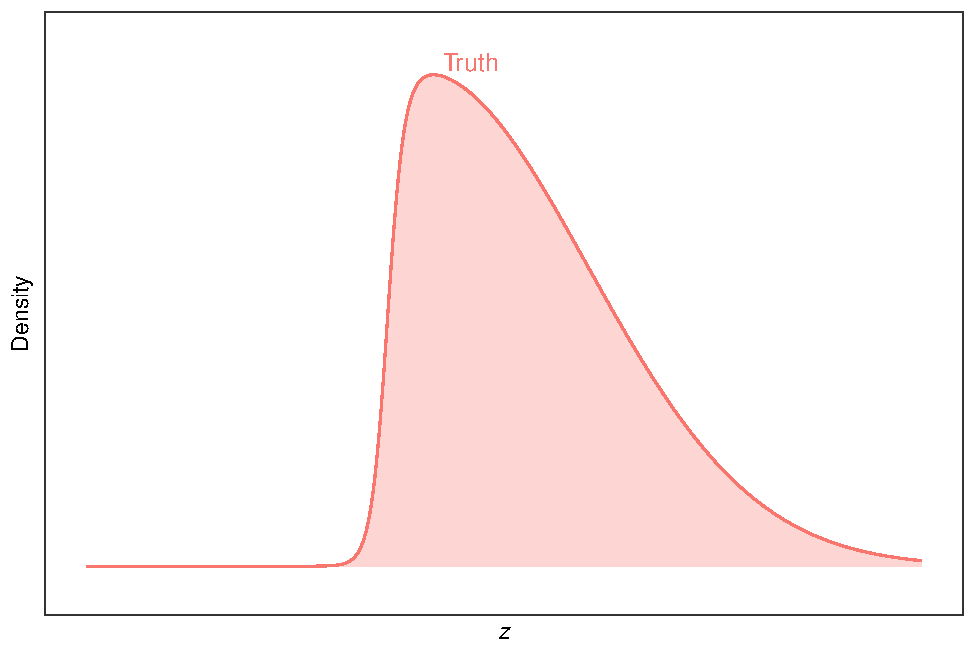
\includegraphics[scale=0.7]{figure/compare1}
%    \end{center}
%  }
%%  \only<2|handout:0>{
%%    \begin{center}
%%      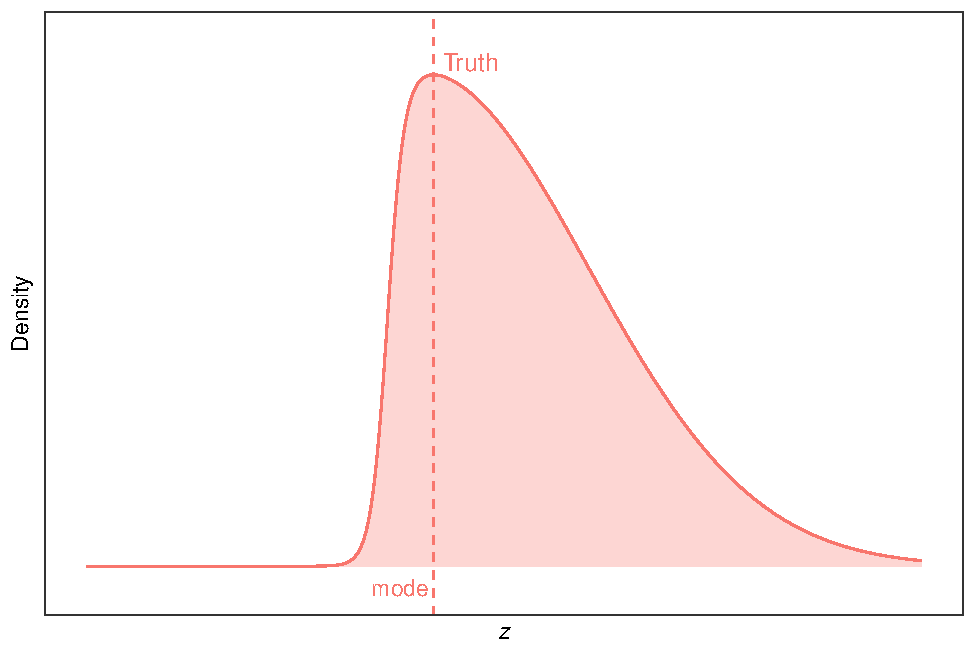
\includegraphics[scale=0.7]{figure/compare2}
%%    \end{center}
%%  }  
%  \only<2|handout:0>{
%    \begin{center}
%      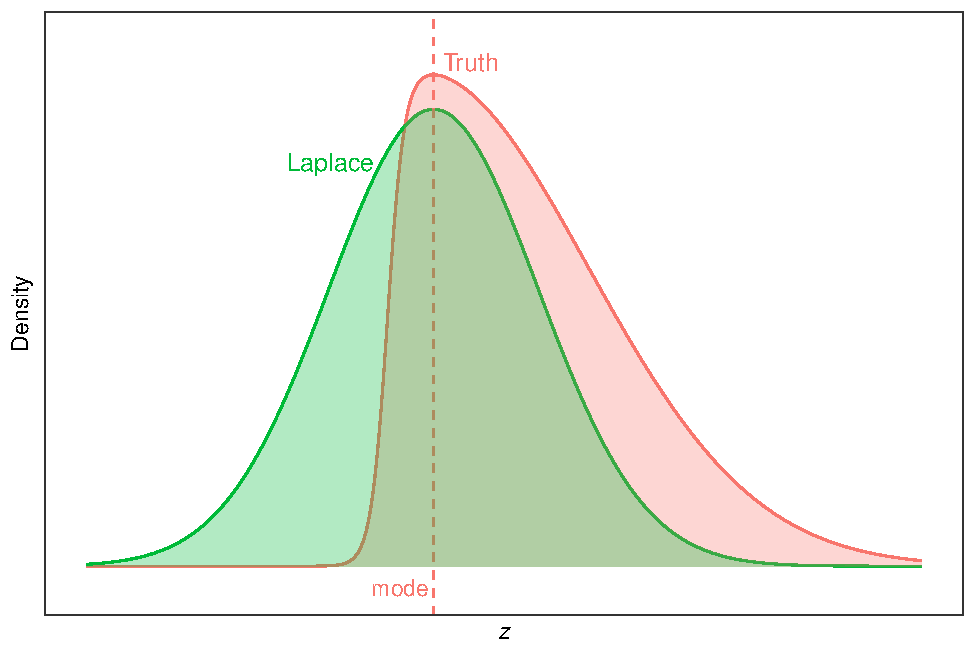
\includegraphics[scale=0.7]{figure/compare3}
%    \end{center}
%  } 
%%  \only<4|handout:0>{
%%    \begin{center}
%%      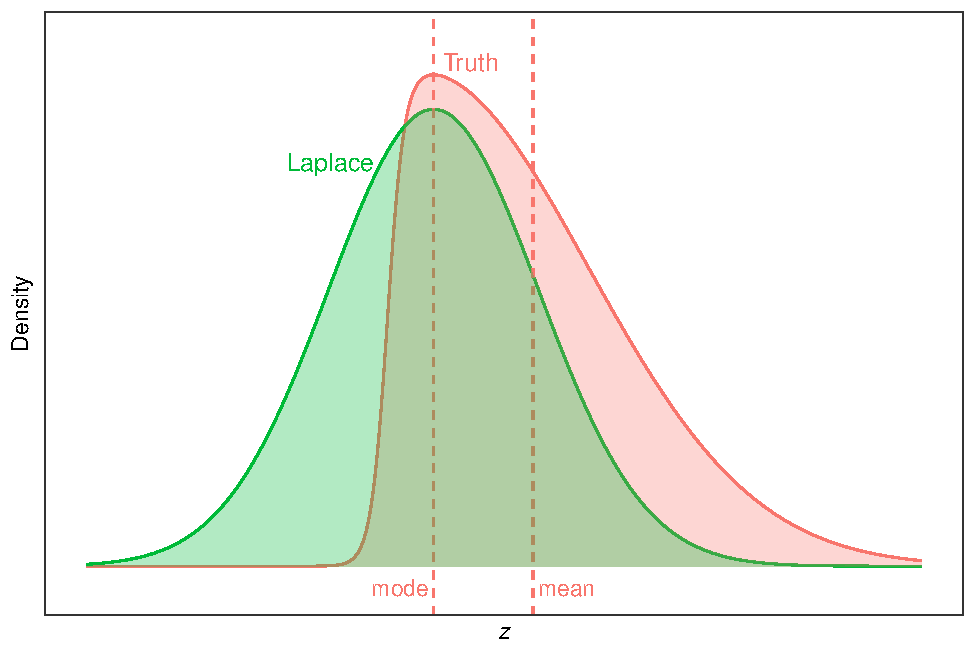
\includegraphics[scale=0.7]{figure/compare4}
%%    \end{center}
%%  } 
%  \only<3|handout:1>{
%    \begin{center}
%      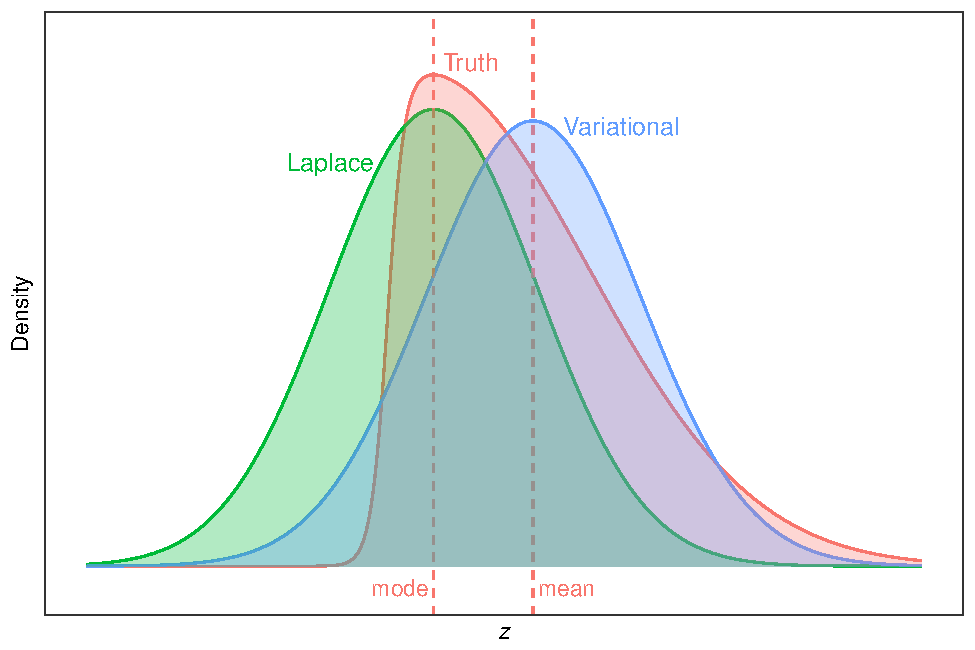
\includegraphics[scale=0.7]{figure/compare5}
%    \end{center}
%  } 
%  
%  \begin{textblock*}{3cm}(.982\textwidth,1.04\textheight)%
%    \hyperlink{summary}{\beamerbutton{back}}      
%  \end{textblock*}
%\end{frame}
%
%\begin{frame}{Comparison of approximations (deviance)}
%  \vspace{-5pt}
%  \begin{center}
%    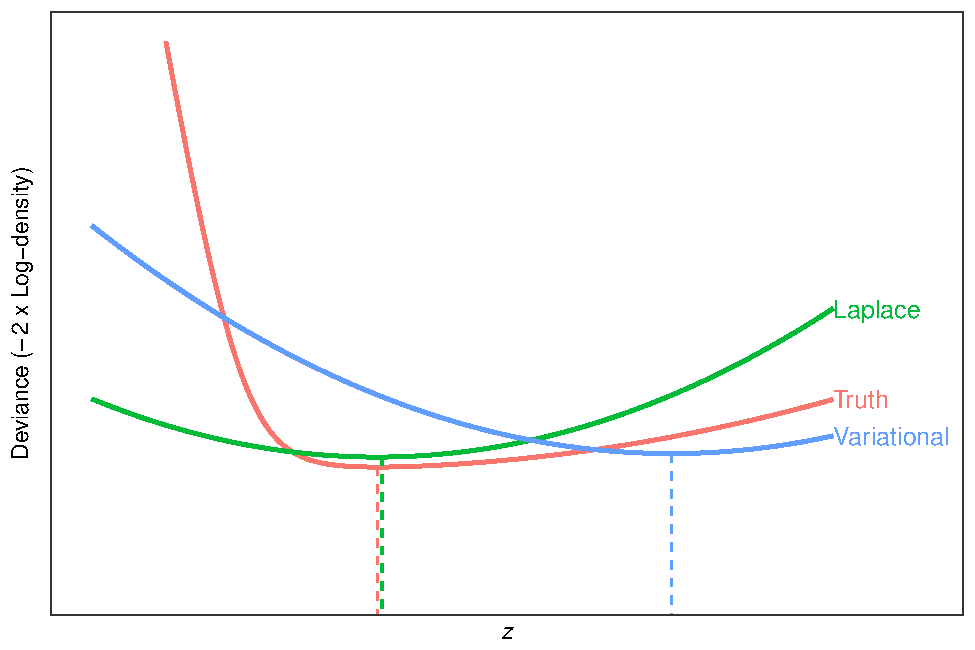
\includegraphics[scale=0.7]{figure/compare6}
%  \end{center}
%
%  \begin{textblock*}{3cm}(.982\textwidth,1.04\textheight)%
%    \hyperlink{summary}{\beamerbutton{back}}      
%  \end{textblock*}  
%\end{frame}

\begin{frame}{Factorised distributions (Mean-field theory)}
%  \blfootnote{\fullcite{Blei2016}}
  \vspace{-20pt}
  \begin{itemize}
    \item<1-> Maximising $\cL$ over all possible $q$ not feasible. Need some restrictions, but only to achieve tractability.
    \item<1-> Suppose we partition elements of $\bz$ into $M$ disjoint groups $\bz = (\bz^{(1)}, \dots, \bz^{(M)})$, and assume
    \[
      q(\bz) = \prod_{j=1}^M q_j(\bz^{(j)}).
    \]
    \item<2-> Under this restriction, the solution to $\argmax_q \cL(q)$ is
    \begin{align}\label{eq:meanfieldsoln}
      \tilde q_j(\bz^{(j)}) \propto \exp\big(\E_{-j}[\log p(\by,\bz)]\big)
    \end{align}
    for $j \in \{1,\dots,m\}$.
    \item<3-> In practice, these unnormalised densities are of recognisable form (especially if conjugate priors are used).
    \vspace{4pt}
  \end{itemize}
\end{frame}

\begin{frame}[label=cavi]{Coordinate ascent mean-field variational inference (CAVI)}
  \vspace{-5pt}
  \begin{itemize}\setlength\itemsep{0.4em}
    \item The optimal distributions are coupled with another, i.e. each $\tilde q_j(\bz^{(j)})$ depends on the optimal moments of $\bz^{(k)}$, $k \in \{1,\dots,M:k \neq j\}$.
    \item One way around this to employ an iterative procedure.
    \item Assess convergence by monitoring the lower bound
    \[
      \cL(q) = \E_{ q}[\log p(\by, \bz)] - \E_{ q}[\log q(\bz)].
    \]
  \end{itemize}
  \vspace{-12pt}
    \begin{center}
    \scalebox{0.9}{
    \begin{minipage}{\linewidth}
  \begin{algorithm}[H]
    \caption{CAVI}\label{alg:cavi}
    \begin{algorithmic}[1]
      \State \textbf{initialise} Variational factors $q_j(\bz^{(j)})$
      \While{$\cL(q)$ not converged}
        \For{$j = 1,\dots,M$}
          \State $\log q_j(\bz^{(j)}) \gets \E_{-j}[\log p(\by,\bz)] + \const$
        \EndFor
        \State $\cL(q) \gets \E_{ q}[\log p(\by, \bz)] - \E_{ q}[\log q(\bz)]$
      \EndWhile
      \State \textbf{return} $\tilde q(\bz) = \prod_{j=1}^M \tilde q_j(\bz^{(j)})$ 
    \end{algorithmic}
  \end{algorithm}
      \end{minipage}%
    }
  \end{center}
%  
%  \begin{textblock*}{3cm}(.89\textwidth,1\textheight)%
%    \hyperlink{varex}{\beamerbutton{example}}      
%  \end{textblock*}
\end{frame}
